\documentclass[tikz,border=10pt]{standalone}
\usepackage{amsmath}
\usepackage{tikz}
\usetikzlibrary{arrows.meta, positioning, calc, shapes.geometric}

\begin{document}
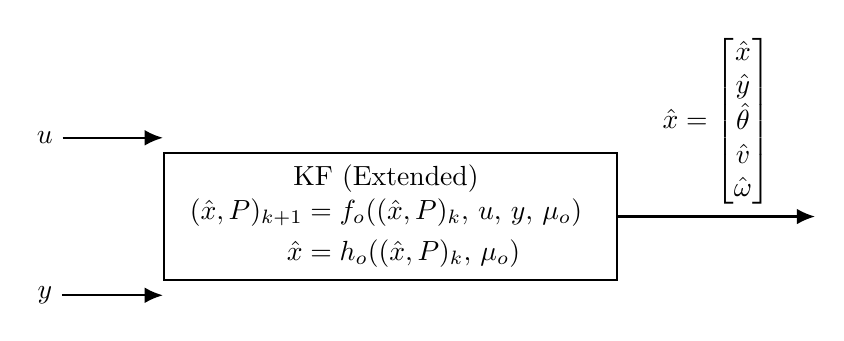
\begin{tikzpicture}[
  block/.style = {draw, thick, minimum height=3em, minimum width=6em, align=center},
  arrow/.style = {thick, -{Latex[width=2mm]}},
  node distance=2.5cm and 2.5cm
]

  % Inputs
  \node (u_in) at (0,1) {$u$};
  \node (y_in) at (0,-1) {$y$};

  % Observer
  \node[block, right=1.5cm of $(u_in)!0.5!(y_in)$] (observer) {
    \begin{tabular}{c}
      KF (Extended)\\
    $\begin{aligned}
      (\hat{x}, P)_{k+1} &= f_o((\hat{x}, P)_k,\,u,\,y,\,\mu_o) \\
      \hat{x} &= h_o((\hat{x}, P)_k,\,\mu_{o})
       \end{aligned}$
    \end{tabular}
  };

  % Inputs
  \draw[arrow] (u_in) -- (observer.west |- u_in);
  \draw[arrow] (y_in) -- (observer.west |- y_in);

  % Output
  \draw[arrow] (observer.east) -- ++(2.5,0) node[midway,above] {$\hat{x} = \begin{bmatrix} \hat{x} \\ \hat{y} \\ \hat{\theta} \\ \hat{v} \\ \hat{\omega} \end{bmatrix}$};

\end{tikzpicture}
\end{document}
